%%
%% Copyright (c) 2022-2023 by Friedemann Bartels
%%
%% This file may be distributed and/or modified under the
%% conditions of the LaTeX Project Public License, either
%% version 1.3c of this license or (at your argument) any later
%% version.  The latest version of this license is in:
%%
%%    http://www.latex-project.org/lppl.txt
%%
%% and version 1.3c or later is part of all distributions of
%% LaTeX version 2008/05/04 or later.
%%

\documentclass[a4paper]{ltxdoc}
\usepackage{microtype}
\usepackage{hyperref}
\usepackage{tikz}
\OnlyDescription
\hypersetup{pdfborder={0 0 0}}
\def\pagelayoutversion{1.0.5}

\begin{document}

\title{
  \Huge The \textsf{pagelayout} class\vskip3mm
  \Large Manual for Version \pagelayoutversion\vskip3mm
  \normalsize\url{https://github.com/friedemannbartels/latex-pagelayout}
}

\author{\href{mailto:mail@friedemannbartels.de}{Friedemann Bartels}}

\maketitle

\tableofcontents

\newpage

\section{Introduction}

When Apple discontinued its photo book feature in Apple Photos, I was missing an easy-to-use photo book application.
In 2020, I started to develop my own solution.
What started with some SVG templates and shell scripts ended up in the pagelayout class, a declarative desktop publishing approach.
\par
With the pagelayout class you can create single- and double-sided documents, create pages with margins, safety margins, and bleed, use templates, align text and graphics in a grid, wrap text across multiple pages and use before pages.
Automatic grid layout and a simple and consistent user interface make it easier than ever to create graphics-rich documents with \LaTeX.
Under the hood the TikZ and tcolorbox packages, ImageMagick and Inkscape are used.

\section{Document}\label{sec:document}

The document arguments described in the following can be either set as a document argument (|\documentclass[twoside]{pagelayout}|) or with a command (|\twoside|) in the preamble.

\DescribeMacro {\documentclass}
Use the class with the |\documentclass|\oarg{arguments}|{pagelayout}| command.
A single sided document is the default.
\begin{figure}[h!]
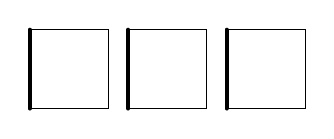
\begin{tikzpicture}
  \draw[black, thin] (0,0) rectangle (1,1);
  \draw[black, line width=1.5pt,line cap=round] (0,0) -- (0,1);
  \draw[black, thin] (1.25,0) rectangle (2.25,1);
  \draw[black, line width=1.5pt,line cap=round] (1.25,0) -- (1.25,1);
  \draw[black, thin] (2.5,0) rectangle (3.5,1);
  \draw[black, line width=1.5pt,line cap=round] (2.5,0) -- (2.5,1);
\end{tikzpicture}
\end{figure}

\DescribeMacro {\twoside}
Using the document argument |twoside| results in a document with left and right pages.
When you create a two-sided document, your document always has an even number of pages.
If you create a document with an odd number of pages, an additional page is automatically inserted.
Two-sided documents start with a right page by default.
\begin{figure}[h!]
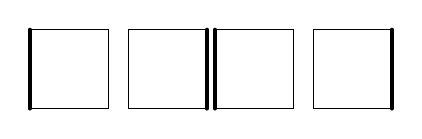
\begin{tikzpicture}
  \draw[black, thin] (0,0) rectangle (1,1);
  \draw[black, line width=1.5pt,line cap=round] (0,0) -- (0,1);
  \draw[black, thin] (1.25,0) rectangle (2.25,1);
  \draw[black, line width=1.5pt,line cap=round] (2.25,0) -- (2.25,1);
  \draw[black, thin] (2.35,0) rectangle (3.35,1);
  \draw[black, line width=1.5pt,line cap=round] (2.35,0) -- (2.35,1);
  \draw[black, thin] (3.6,0) rectangle (4.6,1);
  \draw[black, line width=1.5pt,line cap=round] (4.6,0) -- (4.6,1);
\end{tikzpicture}
\end{figure}

\DescribeMacro {\beginleft}
Use the argument |beginleft| to begin with a left page.
\begin{figure}[h!]
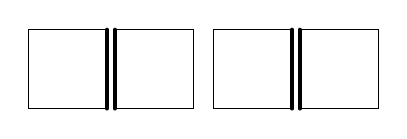
\begin{tikzpicture}
  \draw[black, thin] (0,0) rectangle (1,1);
  \draw[black, line width=1.5pt,line cap=round] (1,0) -- (1,1);
  \draw[black, thin] (1.1,0) rectangle (2.1,1);
  \draw[black, line width=1.5pt,line cap=round] (1.1,0) -- (1.1,1);
  \draw[black, thin] (2.35,0) rectangle (3.35,1);
  \draw[black, line width=1.5pt,line cap=round] (3.35,0) -- (3.35,1);
  \draw[black, thin] (3.45,0) rectangle (4.45,1);
  \draw[black, line width=1.5pt,line cap=round] (3.45,0) -- (3.45,1);
\end{tikzpicture}
\end{figure}

By default, each page is placed on one paper.
\DescribeMacro {\fanfold}
With the |fanfold| argument you can change this behavior so that a left and a right page are placed on one paper.
In this case, the first page is a left one by default.
\begin{figure}[h!]
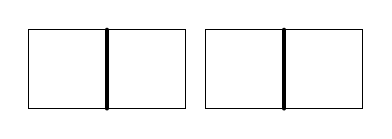
\begin{tikzpicture}
  \draw[black, thin] (0,0) rectangle (1,1);
  \draw[black, thin] (1,0) rectangle (2,1);
  \draw[black, line width=1.5pt,line cap=round] (1,0) -- (1,1);
  \draw[black, thin] (2.25,0) rectangle (3.25,1);
  \draw[black, thin] (3.25,0) rectangle (4.25,1);
  \draw[black, line width=1.5pt,line cap=round] (3.25,0) -- (3.25,1);
\end{tikzpicture}
\end{figure}

\DescribeMacro {\cover}
The |cover| argument is similar to the |fanfold| argument, but only applied to cover pages.
Read more about cover pages in section~\ref{sec:pages}.
\begin{figure}[h!]
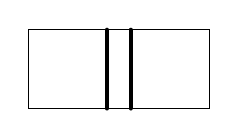
\begin{tikzpicture}
  \draw[black, thin] (0,0) rectangle (2.3,1);
  \draw[black, line width=1.5pt,line cap=round] (1,0) -- (1,1);
(3.25,1);
  \draw[black, line width=1.5pt,line cap=round] (1.3,0) -- (1.3,1);
(3.25,1);
\end{tikzpicture}
\end{figure}

\DescribeMacro {\beginright}
If you want your fanfold document to start with a right hand page, you can use the argument |beginright|.
\begin{figure}[h!]
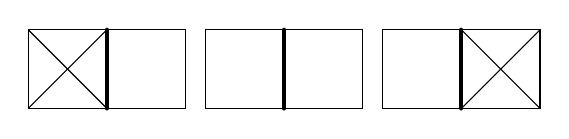
\begin{tikzpicture}
  \draw[black, thin] (0,0) rectangle (1,1);
  \draw[black, thin] (0,0) -- (1,1);
  \draw[black, thin] (0,1) -- (1,0);
  \draw[black, thin] (1,0) rectangle (2,1);
  \draw[black, line width=1.5pt,line cap=round] (1,0) -- (1,1);
  \draw[black, thin] (2.25,0) rectangle (3.25,1);
  \draw[black, thin] (3.25,0) rectangle (4.25,1);
  \draw[black, line width=1.5pt,line cap=round] (3.25,0) -- (3.25,1);
  \draw[black, thin] (4.5,0) rectangle (5.5,1);
  \draw[black, thin] (5.5,0) rectangle (6.5,1);
  \draw[black, thin] (5.5,0) -- (6.5,1);
  \draw[black, thin] (5.5,1) -- (6.5,0);
  \draw[black, line width=1.5pt,line cap=round] (5.5,0) -- (5.5,1);
\end{tikzpicture}
\end{figure}

\subsection{Lengths}\label{subsec:size}

The document lengths described below can be set either as a document argument (|\documentclass[page width=21cm]{pagelayout}|) or by assigning the dimension directly (|\pagewidth=21cm|) in the preamble or in the document.

\DescribeMacro {\pagewidth}
\DescribeMacro {\pageheight}
You can set the lengths |page width| and |page height|.
The default page size is |210mm| by |297mm|.

\DescribeMacro {\bleed}
You can set the |bleed| length.
It applies to all paper edges.
The default bleed is |0mm|.
You can override the bleed for each edge separately by defining the lengths |top bleed|, |inner bleed|, |bottom bleed|, |outer bleed|.
The paper size results from the page size and the bleed.

\DescribeMacro {\safetymargin}
The |safety margin| is the only length that has no influence on the final result.
Its only purpose is to control the safe zone when editing.
It is |0mm| by default and can be configured for each edge by defining |top safety margin|, |inner safety margin|, |bottom safety margin| and |outer safety margin|.

\DescribeMacro {\margin}
\DescribeMacro {\gutter}
You can set the lengths |margin| and |gutter| for the document, for a page (see section~\ref{sec:pages}) or for a grid (see section~\ref{sec:grid}).
The default margin is |20mm|, the default gutter is |0mm|.
Similar to bleed and safety margin, the margin can be defined for each edge individually by setting |top margin|, |outer margin|, |bottom margin| and |inner margin|.

You can create documents with cover pages.
\DescribeMacro {\coverwidth}
\DescribeMacro {\coverheight}
Read more about creating cover pages in section~\ref{sec:pages}.
You can set the lengths |coverwidth| and |coverheight|.
By default, the cover pages are the same size as the inside pages.
If you want to create a cover with a spine, use the |fanfold| or |cover| argument described in section~\ref{sec:document}.
In this case the length |spinewidth| takes effect.
The default spine width is |3mm|.
\par
You can overwrite the bleed and the safety margin for cover pages.
To do this, prefix the respective lengths described above.
For example, define |cover inner bleed| or |cover safety margin|.

\subsection{Page Graphics and Colors}\label{subsec:colors}

You can define a page graphic and a page color with the arguments |page graphic| and |page color|.
Set the argument |color| to define the text color.
These arguments can be defined for the document or for each page (see section~\ref{sec:pages}).
\par
Read how to set the scale and crop of a page graphic with the |\newgraphic| command in section~\ref{sec:content}.

\subsection{Layout Guides}

The layout guides described in the following can be either set as a document argument (|\documentclass[grid]{pagelayout}|) or using a command (|\grid|) in the preamble or the document.
Layout guides can be switched on (|\safezone|) or off (|\nosafezone|).

\DescribeMacro {\grid}
The |grid| argument visualizes the margin and the grid gutters with green lines.
Read more about the grid in section~\ref{sec:grid}.
\DescribeMacro {\safezone}
The |safezone| layout guide shows a red border for the bleed and a thin pink line to indicate the safety margin.
\DescribeMacro {\cuttingmarks}
As an alternative to |safezone|, you can also use |cutting marks| to display cutting marks.
\DescribeMacro {\graphpaper}
Show a graph paper with the |graph paper| argument.

\begin{figure}[h]
\begin{tikzpicture}
  \node[anchor=south west,inner sep=0] (image) at (0,0) {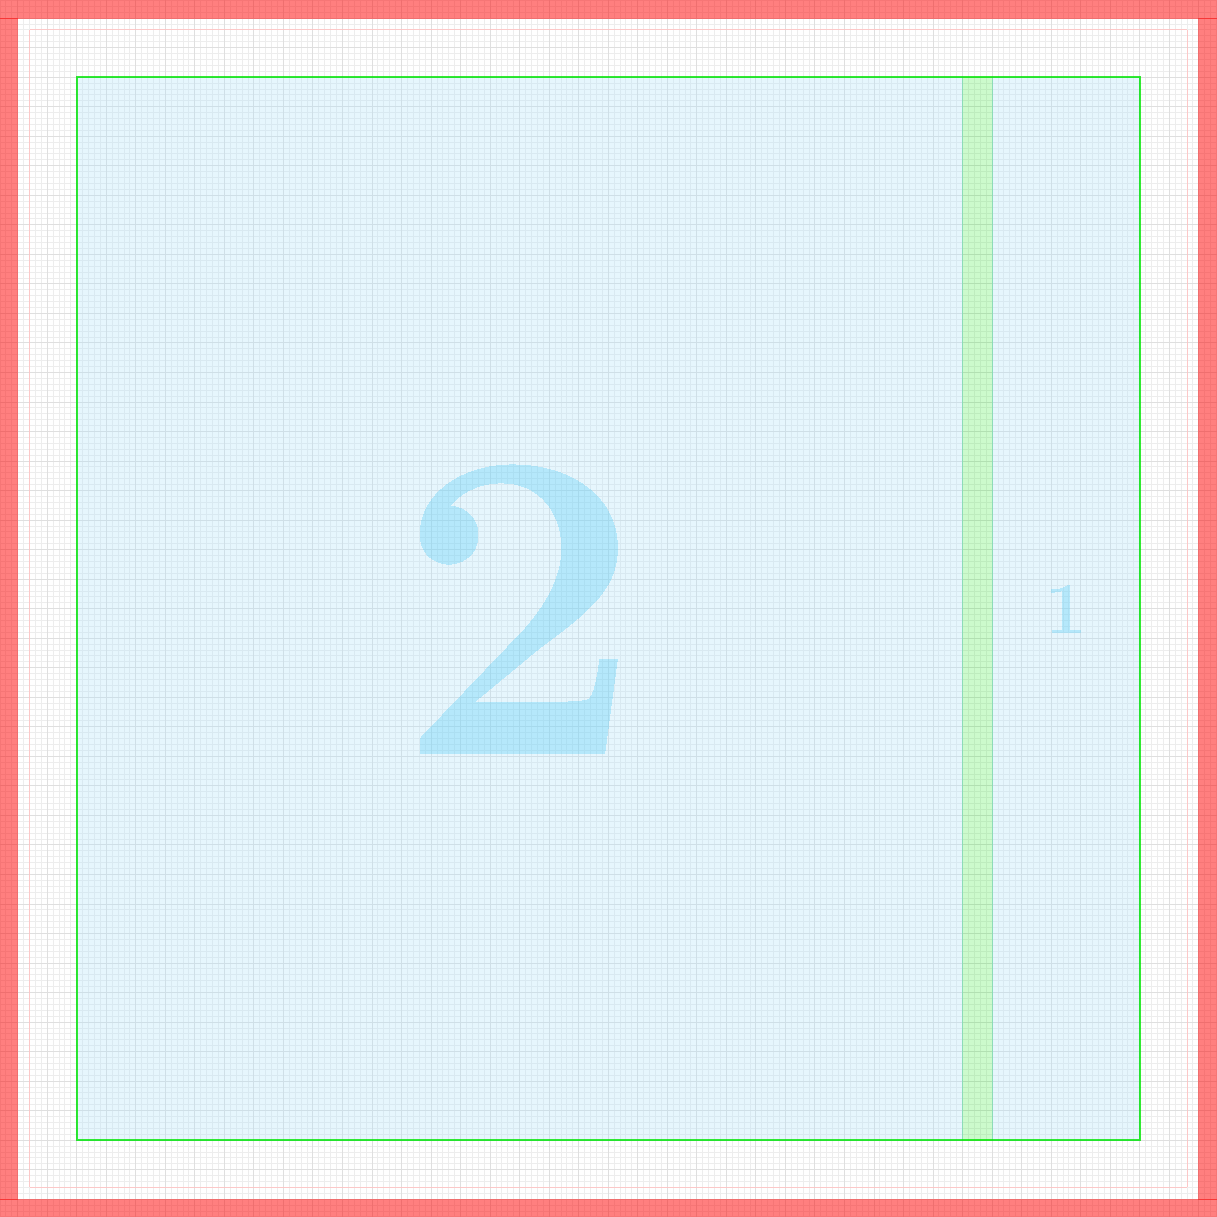
\includegraphics[trim={15cm 16.5cm 0cm 0},clip,scale=1,page=1]{pagelayout-manual-layout-guides.pdf}};
  \node[anchor=south west,text depth=0mm,text width=4cm] (bleed) at (65mm,33mm) {Bleed};
  \draw (bleed) -- ++(-32mm,0);
  \node[anchor=south west,text depth=0mm,text width=4cm] (bleed) at (65mm,27mm) {Safety margin};
  \draw (bleed) -- ++(-35mm,0.0);
  \node[anchor=south west,text depth=0mm,text width=4cm] (margin) at (65mm,21mm) {Margin};
  \draw (margin) -- ++(-43mm,0.0);
  \node[anchor=south west,text depth=0mm,text width=4cm] (gutter) at (65mm,15mm) {Gutter};
  \draw (gutter) -- ++(-70mm,0.0);
  \node[anchor=south west,text depth=0mm,text width=4cm] (placeholder) at (65mm,9mm) {Placeholder};
  \draw (placeholder) -- ++(-50mm,0.0);
  \node[anchor=south west,text depth=0mm,text width=4cm] (graphpaper) at (65mm,3mm) {Graph paper};
  \draw (graphpaper) -- ++(-40mm,0.0);
\end{tikzpicture}%
\end{figure}

\DescribeMacro {\placeholders}
The |placeholders| argument shows template placeholders.
Read more about templates in section~\ref{sec:templates}.
\DescribeMacro {\fillpages}
If you create a document with a cover and a first right hand page, use the |fill pages| argument during editing to add blank pages to get a better impression of the final result.

\subsection{Draft Mode}\label{subsec:draftmode}

The |draft| argument is a shortcut to enable the arguments |placeholders|, |cutting marks| and |fill pages|.
It also speeds up rebuilding the PDF when changing the document.

\section{Pages}\label{sec:pages}

\DescribeMacro {\page}
Create a page with the command |\page|\oarg{arguments}\marg{content}.
You can overwrite the document arguments |margin|, |top margin|, |bottom margin|, |inner margin|, |outer margin|, |gutter|, |page color|, |page graphic| and |color| for each page.

Use the argument |double| to create a double page.
When creating a double page after a left page, a right page is automatically inserted before the double page.
The argument |double| is only recognized for double sided documents.
\par
Use the arguments |front cover| or |back cover| to create a front or back cover.
If you have a back cover and a front cover, the back cover page must be defined first.
If no argument is active, the front cover is placed as the first page and the back cover as the last page of the document.
In this case, the only difference from normal pages is that the cover pages are not counted in the page numbering.
\par
If the argument |fanfold| or |cover| is selected, the back and front covers are laid out on one paper so that the cover is suitable for a book with a hard or soft cover (see section~\ref{sec:document}).
Space is reserved between the back and front covers for the spine.
Set the |spine width| document argument as described in section~\ref{subsec:size}.
\par
With the arguments |hpos| and |vpos| you can set the default grid alignment for a page.
Read more about the grid in the next section.

\DescribeMacro {\setpagecolor}Alternativly to the argument you can use the command |\setpagecolor|\marg{color} to set the page color for all following pages.

\DescribeMacro {\setpagegraphic}With the command |\setpagegraphic|\oarg{arguments}\marg{name} you can define a page graphic for all following pages.
The name references a graphic version created with the |\newgraphic| command (see section~\ref{sec:content}).
If no graphic version with the given name exists, the command uses the name as the file name.
You can change the clipping by defining relative decimal values for the arguments |scale| (>1), |hpos| and |vpos| (0-1).

\DescribeMacro {\newbeforepage}With the command |\newbeforepage|\marg{name}\marg{content} you can create a reusable page layer, that can be set before pages.
\DescribeMacro {\setbeforepage}
Use the command |\setbeforepage|\marg{name} to define a before page for all following pages or use the page argument |before page| to specify a before page for a individual page.

\DescribeMacro {\ifleftpage}
\DescribeMacro {\ifrightpage}
Use the condition |\ifleftpage|\marg{content} and |\ifrightpage|\marg{content} to check for the current page alignment.

\DescribeMacro {\leftpage}
Within a page scope you can use the |\leftpage|\marg{content} command to place content only on a left page.
In comparison to the |\ifleftpage|\marg{content} condition, the command sets a grid for a single page.
That way you can combine single with double page layouts.
\DescribeMacro {\rightpage}
Accordingly you can use the |\rightpage|\marg{content} command.

\section{Grid}\label{sec:grid}

The grid allows you to create rows with cells.
You can define width and height relations between rows and cells.
All definitions are relative.
The size and position results from these relations and the configured dimensions page width, page height, margin and gutter.

\DescribeMacro{\setgrid}
Create a grid with the command |\setgrid|\oarg{arguments}\marg{config}.
The grid configuration is a nested list of rows and cells.
A cell is defined by a number that describes the width ratio to the other cells in the row.
The default grid describes a row with one cell:

\begin{verbatim}
  \setgrid{
    {{}}}
\end{verbatim}

You can define a width relation between cells by adding a integer value for each cell:

\begin{verbatim}
  \setgrid{
    {{1}{2}}}
\end{verbatim}

With an optional integer value for each row you can set a height relation between rows:

\begin{verbatim}
  \setgrid{
    {[2]{1}{2}}
    {[1]{1}{2}}}
\end{verbatim}

You can set an aspect ratio for a cell by adding a |!| to the width.
This way the aspect ratio is defined by the width of the cell and the height of the row.
If all cells in a row have a fixed aspect ratio, the aspect ratio of the row is fixed too.
In the following, a row with only fixed cells is named a fixed row.
Because the height of a fixed row is determined by the aspect ratios of the cells, the height relation to the flexible rows is broken.
In this case, you can force a height relation between flexible and fixed rows by adding a |!| to the height of the flexible row.
In the following, a row with a forced height is named a forced row.

The example defines a first fixed row with one cell and an aspect ratio of 3:2.
The height of the second row is forced half of the height of the first row.
The cells in the second row share the available width in the ratio one to two:

\begin{verbatim}
  \setgrid{
    {[2]{3!}}
    {[1!]{1}{2}}}
\end{verbatim}

If the height of fixed and forced rows exceeds the available height, the grid shrinks to fit the available space.
The defined aspect ratios of the cells are preserved and the grid is centered horizontally.
In this case you can define the |hpos| argument to align the grid horizontally.
A value of |0| aligns the grid to the left, a value of |1| aligns the grid to the right.
The default is a value of |0.5|.

If the height of fixed and forced rows is less than the available height, all flexible rows share the excess height.
If there are no flexible rows, the grid is centered vertically.
In this case you can define the |vpos| argument to align the grid vertically.
A value of |0| aligns the grid to the top, a value of |1| aligns the grid to the bottom.
The default is a value of |0.5|.

As for a document or a page you can set |margin| and |gutter| arguments for a specific grid.
With the arguments |width|, |height|, |x| and |y| you can override the intrinsic grid size and position.
When overriding the grid size and position, you can calculate with the intrinsic values, for example |x=\x-1cm|.

\subsection{Placing Content}

The grid aligns content (see section~\ref{sec:content}) automatically in the given grid cells.
To set the position of a content box manually use the command |\place|\marg{fromrow fromcell torow tocell}.
\DescribeMacro{\place}
To place content in the first row and first cell use the command |\place{0 0 1 1}| before the content.
The definded place applies only for the following content box.
The next boxes are then again placed with auto layout.
\par
The command accepts decimals.
That allows you to place content everywhere within the grid.
The |gutter| is taken into account when calculating the positions.

\section{Content}\label{sec:content}

\subsection{Text}

\DescribeMacro{\text}
With the command |\text|\oarg{arguments}\marg{text} you can place text.
Align the text vertically with the |center| and |bottom| arguments.
\par
The |\text| command uses the package tcolorbox and accepts tcolorbox arguments, for example to set text, frame or background color and transparency.
The tcolorbox behaves slightly diffenrent then the standalone version: spacings, rules and background are removed by default.
You can change the behaviour with the tcolorbox command |\tcbset|\marg{arguments}.
Also the |arc| arguments behaves different: if you set the |arc| to |0pt| the |outer arc| is also set to |0pt|.
\par
Add the argument |breakable| to break text over multiple boxes and pages.
\DescribeMacro{\usetext}
Use the command |\usetext|\oarg{name} to place the following text boxes in the grid.
If you want to use multiple breakable text boxes you can initialize the text with the |name| argument and define a name that you then can pass to the |\usetext| argument.
Breakable text boxes may have different heights and positions.
To align the baselines use the |baselinesnap| argument and set the baseline dimension, for example |baselinesnap=\baselineskip|.
\par
The |\text| command accepts the arguments |shadow|, |shadow size|, |shadow color|, |shadow opacity|, |shadow xshift|, |shadow yshift|, |border|, |border width|,\break |border color| and |border radius|.
Read more about shadows and borders in section~\ref{subsec:borders}.

\subsection{Graphics}

\DescribeMacro{\newgraphic}
Create a reusable graphic version with the |\newgraphic|\marg{name}\marg{arguments} command.
Define the arguments |scale| (>1), |hpos| and |vpos| (0-1) to set the clipping of the graphic.
With the argument |file| you can link a file.
If no file is defined, the name is used as the file name.

\DescribeMacro{\graphic}
The command |\graphic|\oarg{arguments}\marg{name} places a graphic.
The name references a graphic version created with the command |\newgraphic|.
If no graphic version with the given name exists, the command uses the name as the file name.

The graphic is scaled to fit in the content box.
If the aspect ratio of the graphic differs from that of the defined content box, the graphic is cropped.
You can change the cropping by defining relative decimal values for the arguments |scale| (>1), |hpos| and |vpos| (0-1).
With the |orientation| argument you can set the Exif orientation flag (1-8).
To flip a graphic horizontally or vertically use the arguments |hflip| or |vflip|.
Same as the |\text| command, the |\graphic| command accepts the |border| and |shadow| arguments described in section~\ref{subsec:borders}.

\DescribeMacro{\graphicspath}
You can use the command |\graphicspath|\marg{dir-list} of the graphics package to specify a list of directories in which to search for graphic files.

\subsection{Other}

\DescribeMacro{\xput}
The command |\xput|\marg{code} is an easy way to place arbitrary content in the grid.
Within the code block the dimensions |\width| and |\height| represent the size of the content area and can be used to create graphics, that fit and adapt to the available size.
\par
\DescribeMacro{\tikzgraphic}
The command |\tikzgraphic|\marg{tikz code} works like the |\xput| command, but wraps your input in a |tikzpicture|.

\subsection{Shadows and Borders}\label{subsec:borders}

Text and graphic content can be placed with a border or a shadow.
You can define a border or shadow for a specific content box by using the arguments |border width|, |border color|, |border radius| to add a border or |shadow size|, |shadow color|, |shadow opacity|, |shadow xshift|, |shadow yshift| to add a shadow.
\par
\DescribeMacro{\newborder}
\DescribeMacro{\newshadow}
Define a reusable border or shadow with the |\newborder|\marg{name}\marg{arguments} or |\newshadow|\marg{name}\marg{arguments} commands.
Apply the border or shadow to |\text| or |\graphic| with the argument |border| or |shadow|.
\par
\DescribeMacro{\setborder}
\DescribeMacro{\setshadow}
To set a border or shadow within a page or document scope, use the commands |\setborder|\oarg{arguments}\marg{name} or |\setshadow|\oarg{arguments}\marg{name}.

\section{Templates}\label{sec:templates}

\DescribeMacro{\newtemplate}
With the command |\newtemplate|\marg{name}\marg{layout} you can create a reusable layout.
Creating a template works the same way as creating a page.
In addition to graphics and text you can define placeholders.
\DescribeMacro{\placeholder}
Use the command |\placeholder|\marg{fromrow fromcell torow tocell} to define a content area that can later be filled with a text or a graphic.

\DescribeMacro{\template}
Use a template with the command |\template|\oarg{arguments}\marg{name}\marg{content}.
The available arguments are the same as for pages.

The command |\template| comes with an easy way to generate templates by using a name pattern.
For example the template name \textit{sp} creates a template with a square and a portrait format placeholder.
In this case the letter |s| specifies a square (1:1) and the letter |p| a portrait (2:3) format placeholder.
Use the letter |l| to define a landscape ratio (3:2), |g| for golden ratio (5:3), |o| for golden upright ratio (3:5), |w| for wide ratio (2:1) or |f| for a flexible ratio.
With the character |-| you can start a new row.
Within a row you can mix the fixed placeholders (|s|, |p|, |l|, |g|, |o|, |w|) or use only flexible placeholders~(|f|).

\section{Image Optimization}\label{sec:optimization}

\DescribeMacro{\optimize}
With the command |\optimize|\oarg{arguments} you can enable image optimization.
When enabled, JPG and PNG images are croped, resized and cached.
This results in fast rebuilds when changing the document.
You can set the arguments |density|, |quality|, |unsharp| and |downsample threshold|.
The |density| argument takes a number of the pixels per inch (default |300|), the |quality| argument takes numbers between 1 and 100, the |unsharp| argument an ImageMagick unsharp configuration (default |2x1|) and the |downsample threshold| a decimal value greater or equal 1 (default |1.2|).
The |unsharp| argument can also be applied for individual graphics.
\par
If you use image optimization and change the original graphics files, you must delete the cached versions so that the cache will update.
\DescribeMacro{\import}
The |\import| command helps you to streamline this process.
When enabled, you need an import directory in which to place the modified files.
When the document is created, the files are moved to your image directory and the corresponding cached versions are automatically regenerated.
The import directory is either the directory \emph{import} in your working directory.
Or you can set a system wide import directory by defining the shell variable |PAGELAYOUT_IMPORT_DIRECTORY|.
\par
\DescribeMacro{\preflight}
Use the |\preflight| command to proof the image resolution.
If images have a final resolution less then 300 ppi you get a warning, if less then 200 ppi you get an error.
With preflight enabled the maximum possible resolution is shown next to each graphic.

\end{document}
